
\chapter{Classification}
\label{ch:capitolo3}
Classification was performed on the available training set using three different algorithms: K-NN (\textit{K-Nearest Neighbours}), Naïve Bayes and Decision Trees.
The target variables chosen for this task are 2: \texttt{titleType} and \texttt{has\_LowEngagement}.
These will be discussed in more detail in the corresponding sections below.
%%%%%%%%%%%%%%%%%%%%%%%%%%%%%%%%%%%%%%%%%%%%%%%%%% DA VEDERE SE METTERE SOLO QUESTO AL POSTO CHE IN OGNUNA DELLE SEZIONI%%%%%%%%%%%%%%%%%%%%%%%%%%%%%%%%%%%%%%%%%%%%%%%%%
% For K-NN and Naïve Bayes, a portion of the training set (referred to as the validation set) was used to select the best hyperparameters for the first model (used as an external validation 
% after internal cross-validation with RandomizedSearch) and to choose the best feature set for the second one. 
% Instead, to identify the optimal hyperparameters for Decision Trees, a Randomized Search was performed
% using Repeated Stratified 5-Fold Cross-Validation with 10 repeats on the training set for binary classification, and 5 repeats for multiclass classification, both optimized for the macro-averaged F1-score.\\

% After training, the models were evaluated on the test set using standard performance metrics. 

%%%%%%%%%%%%%%%%%%%%%%%%%%%%%%%%%%%%%%%%%%%%%%%%%%%%%%%%%%%%%%%%%%%%%%%%%%%%%%%%%%%%%%%%%%%%%%%%%%%%%%%%%%%%%%%%%%%%%%%%%%%%%%%%%%%%%%%%%%%
\section{Binary classification}\label{sec:binary_classification}
The binary target variable used in this task, \texttt{has\_LowEngagement}, was specifically defined for this purpose. 
It identifies records where the \texttt{numVotes} attribute is less than 100.\\

An analysis of semantically related features was run to decide whether to discard any.
\texttt{userReviewsTotal} has a 75\% correlation with
\texttt{numVotes}, while \texttt{criticReviewsTotal} has 67\% correlation.
Due to its semantic similarity with \texttt{numVotes}, \texttt{userReviewsTotal} was discarded for this task.
In contrast, \texttt{criticReviewsTotal} was retained as it was deemed to provide distinct and complementary information. 
Moreover, its correlation with other features was not considered sufficiently high to make the problem trivial.\\

An important aspect of the chosen binary classification task is the class imbalance, with 10287 records
classified as \textit{Low Engagement} and 4668 as \textit{High Engagement} in the training set.
This imbalance was taken into account during model training and evaluation, with a focus on
macro-averaged F1-score to mitigate its impact on the results.\\

\subsection{K-NN - Binary Classification}
\begin{figure}[H]
    \centering
    \begin{minipage}[t]{0.60\textwidth}
        \vspace{0pt}
        The features used for the K-NN algorithm were normalized, as the model is sensitive to unscaled values: log-transformation (when needed) and StandardScaler were applied to data. 

        Then, to perform this task, care was taken in selecting the appropriate type and amount of features to avoid unnecessary increased dimensionality.
    
        For example, to provide the model with information about the origin of the titles, without introducing all 7 \texttt{countryOfOrigin\_[continent code]} attributes, only \texttt{countryOfOrigin\_freq\_enc} was kept. 
        The remaining variables of the dataset were maintained as they offered diverse and non-redundant insights.\\

       For this algorithm, a portion of the training set was held out as a validation set to enable external validation after internal cross-validation. 
       A randomized hyperparameter search was indeed performed on the reduced training set, with each configuration evaluated using stratified 5-fold cross-validation. 
       This process aimed to identify the optimal value of \textit{k} and explore additional algorithm parameters. 
       The best configuration found is: \texttt{weights: 'uniform', n\_neighbors: 9, metric: 'cityblock'}, which achieved the highest accuracy on the selected feature set.\\

        The resulting model shows solid performance, achieving a test accuracy of 0.85. As expected, it performs better on the \textit{Low Engagement} class, with a high recall (0.94) and F1-score (0.89). 
        In contrast, the \textit{High Engagement} class is more challenging for the model; while precision is reasonable (0.83), recall (0.65) indicates that a significant number of instances are misclassified as 
        \textit{Low Engagement}.
    \end{minipage}
    \hfill
    \begin{minipage}[t]{0.35\textwidth}
        \vspace{0pt}
        \centering
        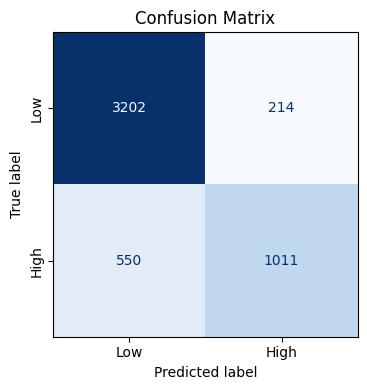
\includegraphics[width=\linewidth]{plots/knn_binary_confmatrix.png}
        \captionsetup{justification=centering, width=0.90\linewidth}
        \caption{K-NN binary classification}
        \label{fig:binary_knn_confusion_matrix}
    \end{minipage}
\end{figure}
% \vspace{-0.8em} % <-- riduce lo spazio dopo la figura

This analysis is reflected in the confusion matrix in Figure~\ref{fig:binary_knn_confusion_matrix}, where 550 out of 1561 \textit{High Engagement} samples were incorrectly labeled as \textit{Low Engagement}.\\

To summarize, the macro average F1-score is 0.81 suggesting that the model maintains a balanced performance across both classes.

% \begin{figure}[H]
%     \centering
%     \begin{minipage}[t]{0.60\textwidth}
%         \vspace{0pt}
%         \small
%         To perform this task using the K-NN algorithm, care was taken in selecting the appropriate type and amount of features to avoid unnecessary increased dimensionality. 
%         For example, to provide the model with information about the origin of the titles, without introducing all 7 \texttt{countryOfOrigin\_[continent code]} attributes, only \texttt{countryOfOrigin\_freq\_enc} was kept. 
%         The remaining variables of the dataset were maintained as they offered diverse and non-redundant insights.\\

%         Then, a randomized hyperparameter search (each configuration evaluated with a stratified 5-fold cross-validation) was performed to identify the proper value of \textit{k}. 
%         This process included the exploration of additional parameters of the algorithm, resulting in: \texttt{weights:'uniform', n\_neighbors:9, metric:'cityblock'}, as it provided the best performance for the selected feature set.\\
%     \end{minipage}
%     \hfill
%     \begin{minipage}[t]{0.35\textwidth}
%         \vspace{0pt}
%         \centering
%         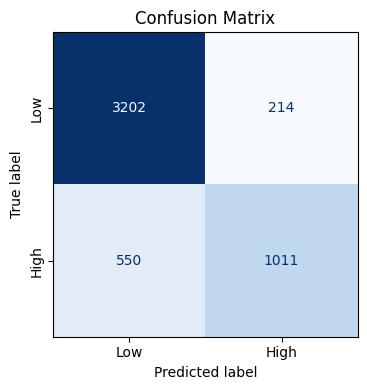
\includegraphics[width=\linewidth]{plots/knn_binary_confmatrix.png}
%         \captionsetup{justification=centering, width=0.90\linewidth}
%         \caption{Confusion matrix - K-NN binary classification}
%         \label{fig:binary_knn_confusion_matrix}
%     \end{minipage}
% \end{figure}
% The resulting model shows solid performance, achieving a test accuracy of 0.85. As expected, it performs better on the \textit{Low Engagement} class, with a high recall (0.94) and F1-score (0.89). 
% In contrast, the \textit{High Engagement} class is more challenging for the model; while precision is reasonable (0.83), recall (0.65) indicates that a significant number of instances are misclassified as 
% \textit{Low Engagement}. This analysis is reflected in the confusion matrix in Figure~\ref{fig:binary_knn_confusion_matrix}, where 550 out of 1561 \textit{High Engagement} samples were incorrectly labeled as \textit{Low Engagement}.\\

% However, the macro average F1-score is 0.81 suggesting that the model maintains a balanced performance across both classes.




% To perform this task using the K-NN algorithm, care was taken in selecting the appropriate type and amount of features to avoid unnecessary increased dimensionality. 
% For example, to provide the model with information about the origin of the titles, without introducing all 7 \texttt{countryOfOrigin\_[continent code]} attributes, only \texttt{countryOfOrigin\_freq\_enc} was kept. 
% The remaining variables of the dataset were maintained as they offered diverse and non-redundant insights.\\
% Then, a randomized hyperparameter search (each configuration evaluated with a stratified 5-fold cross-validation) was performed to identify the proper value of \textit{k}. 
% This process included the exploration of additional parameters of the algorithm, resulting in: \texttt{{weights:'uniform', n\_neighbors:9, metric:'cityblock'}}, as it provided the best performance for the selected feature set.\\
% The resulting model shows solid performance, achieving a test accuracy of 0.85. 
% As expected, it performs better on the \textit{Low Engagement} class, with a high recall (0.94) and F1-score (0.89). 
% In contrast, the \textit{High Engagement} class is more challenging for the model; while precision is reasonable (0.83), recall (0.65) indicates that a significant number of instances are misclassified as 
% \textit{Low Engagement}. This analysis is reflected in the confusion matrix in Figure~\ref{fig:binary_knn_confusion_matrix}, where 550 out of 1561 \textit{High Engagement} samples were incorrectly labeled as \textit{Low Engagement}.
% \begin{figure}[H]
%     \centering
%     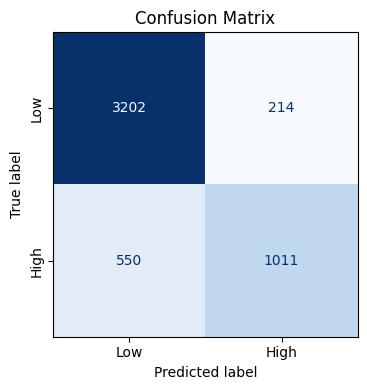
\includegraphics[width=0.35\linewidth]{plots/knn_binary_confmatrix.png}
%     \captionsetup{justification=centering, width=0.9\linewidth}
%     \caption{Confusion matrix - K-NN binary classification}
%     \label{fig:binary_knn_confusion_matrix}
% \end{figure}
% However, the macro average F1-score is 0.81 suggesting that the model maintains a balanced performance across both classes.





\subsection{Naïve Bayes - Binary Classification}
% For Naïve Bayes, a portion of the training set (referred to as the validation set) was used to select the best hyperparameters for the first model (used as an external validation 
% after internal cross-validation with RandomizedSearch) and to choose the best feature set for the second one.
To use Categorical Naïve Bayes, specific preprocessing steps were required: continuous attributes were discretized using semantically meaningful binning and \textbf{Country\_orig} feature was binarized into a (0 / >0) format; 
however, only the from\_America\_bin  and from\_Europe\_bin were used for this particular task. 
All binning strategies applied here are consistent with those described in Subsection X of pattern mining section. 
Finally, the resulting categorical features were numerically encoded using OrdinalEncoder, as required by the CategoricalNB.\\
The results show good classification performance with an overall accuracy of 0.83, a solid outcome given the simplicity of the NB model.
However, differences between classes emerged: the low engagement class performed better, with precision 0.87, recall 0.89, and F1 score 0.88, while the high engagement class had lower results 
(precision of 0.74, recall of 0.70 and F1 score of 0.72), 
Actually, the model struggles more to identify high engagement examples, as confirmed by the low recall (0.70) and by the 481 false negatives in the confusion matrix. 
Conversely, the low engagement class is recognized with greater reliability, with 3063 correct predictions out of 3416.
Finally, the macro F1 average of 0.80 indicates a good balance overall, but some difficulty remains in handling the minority class.
\begin{figure}[H]
    \centering
    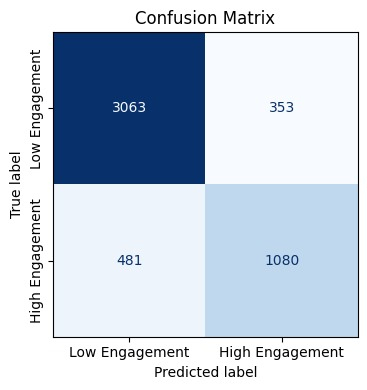
\includegraphics[width=0.30\linewidth]{plots/nb_binary_confmatrix.jpg}
    \captionsetup{justification=centering, width=0.9\linewidth}
    \caption{Naïve Bayes binary classification}
    \label{fig:nb_binary}
\end{figure}


\subsection{Decision Trees - Binary Classification}
For explainability purposes, features were not normalized nor transformed for the Decision Tree model,
as it does not require such preprocessing because it's not based on distance measures, but rather on
decision thresholds.\\

To identify the optimal hyperparameters, a Randomized Search was performed
using Repeated Stratified 5-Fold Cross-Validation with 10 repeats on the training set, optimized for
the macro-averaged F1-score.
The best configuration found used Gini index as the splitting criterion,
a maximum tree depth of 26, and a minimum of 3 samples per leaf.
The obtained decision tree is shown in figure~\ref{fig:binary_dt}.
\begin{figure}[H]
    \centering
    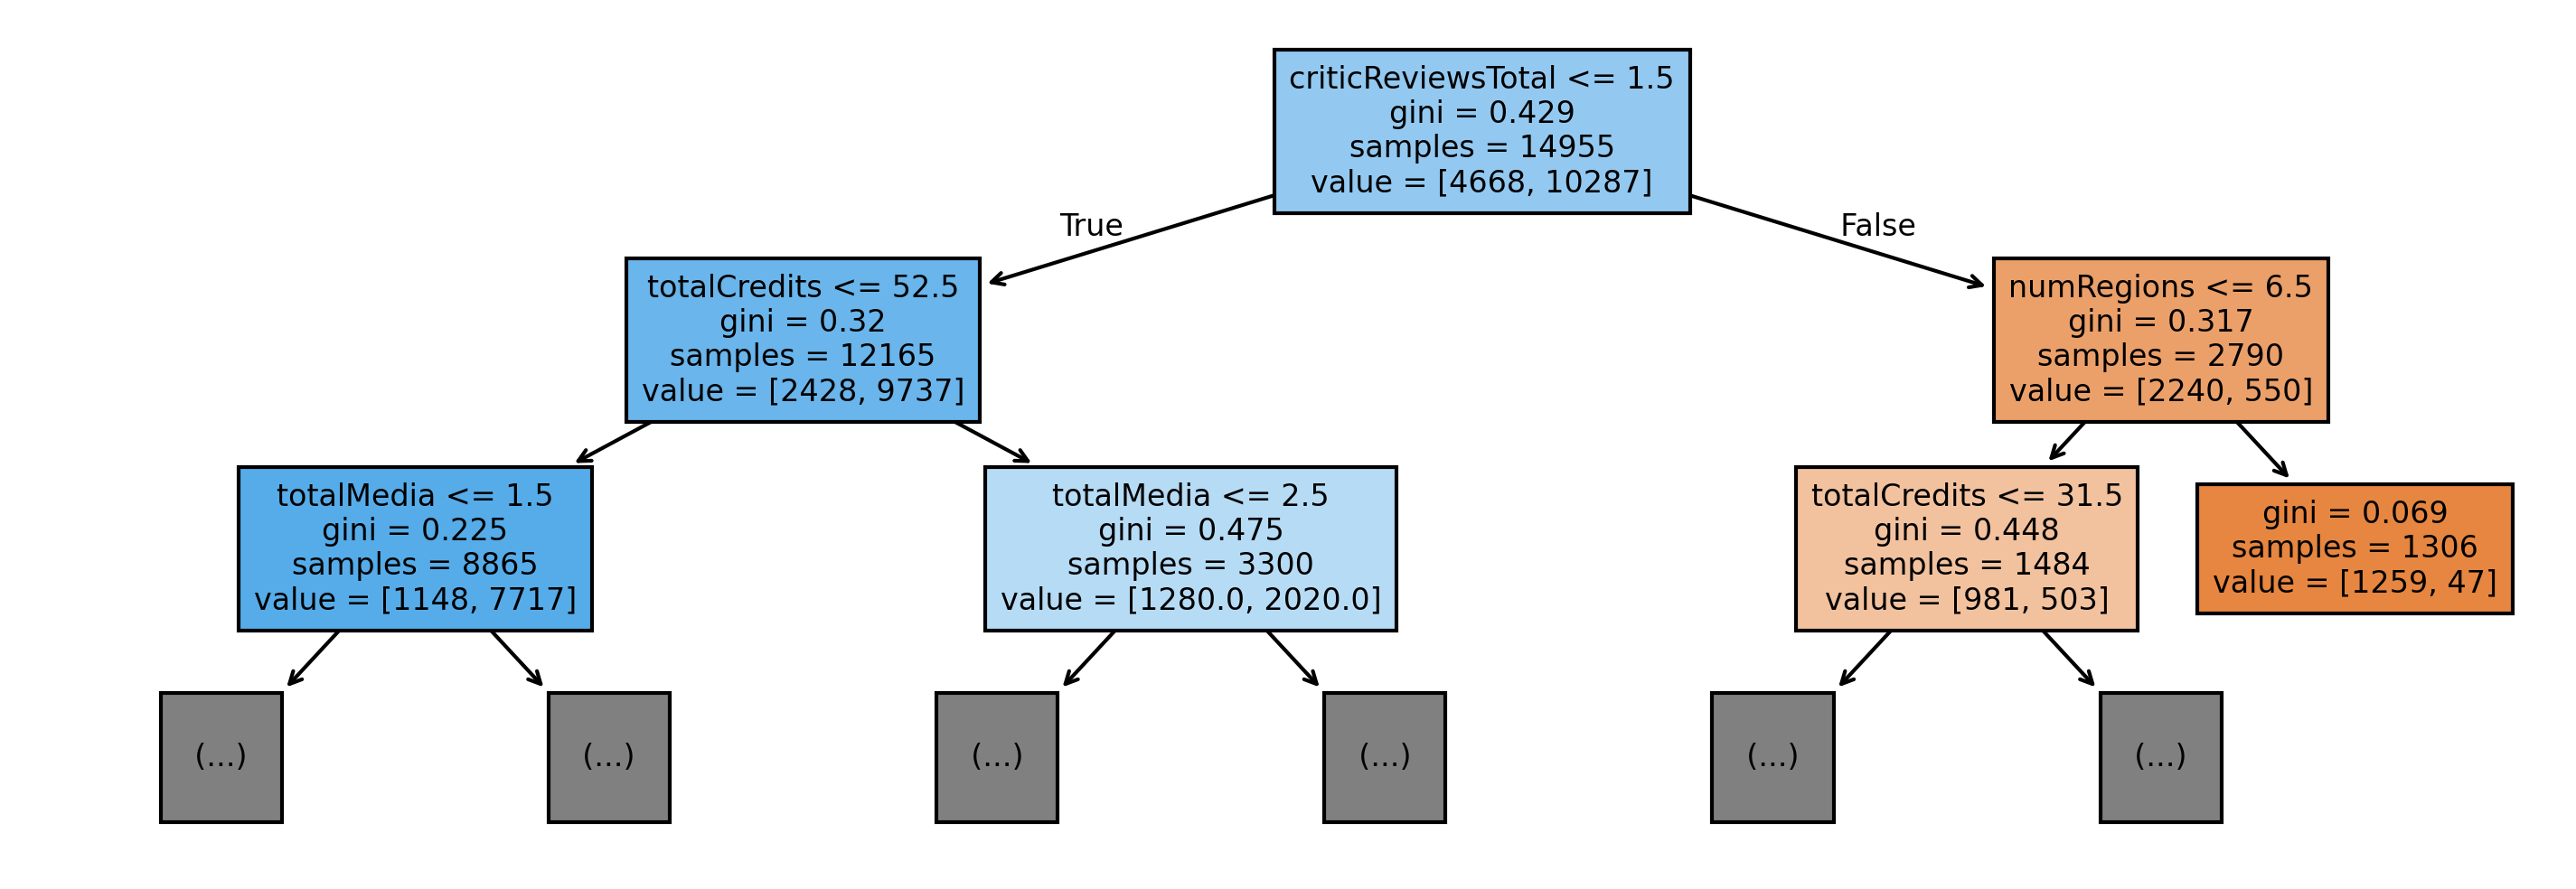
\includegraphics[width=0.8\linewidth]{plots/binary_dt.png}
    \captionsetup{justification=centering, width=0.9\linewidth}
    \caption{Decision Tree for binary classification}
    \label{fig:binary_dt}
\end{figure}

Unsurprisingly, the most important feature for the model was \texttt{criticReviewsTotal},
which amounted to 0.6 in the feature importance ranking. The following other 3 more important
features were \texttt{totalCredits} (0.15), \texttt{totalMedia} (0.10) and \texttt{numRegions} (0.09).
These four features take up around 93\% of the total feature importance, and are all present in the first
two splits shown in the Decision Tree.\\
% Classification performance is summarized in Table~\ref{tab:binary_classification_report}.

% \begin{table}[H]
%     \centering
%     \begin{tabular}{lcccc}
%         \toprule
%         \bf{Class} & \bf{Precision} & \bf{Recall} & \bf{F1-score} & \bf{Support} \\
%         \midrule
%         \bf{Low engagement} & 0.86 & 0.90 & 0.88 & 3416 \\
%         \bf{High engagement} & 0.75 & 0.69 & 0.72 & 1561 \\
%         \midrule
%         \bf{Macro avg} & 0.81 & 0.79 & 0.80 & \\
%         \bf{Weighted avg} & 0.83 & 0.83 & 0.83 & \\
%         \midrule
%         % & & \textbf{Train} & \textbf{Test} & \\
%         % \midrule
%         \bf{ROC AUC} & & & 0.87 & \\
%         \bf{Accuracy}  &  & & 0.83 & \\
%         \bottomrule
%     \end{tabular}
%     \caption{Classification report for binary classification}
%     \label{tab:binary_classification_report}
% \end{table}
Train performance was overall similar to the test performance; in particular, the respective accuracies
were of 0.83 and 0.84, and macro-F1 scores were 0.82 and 0.80.
In any case, post-pruning was tested, but did not yield any performance improvement, and was therefore
not applied.
The \textit{High Engagement} class showed low Recall values (0.71 on train set, 0.68 on test set).
This might be a consequence of class imbalance, as well as poor separability of the two classes.
This assumption is further supported by the
Precision scores of the class (0.78 on train, 0.75 on test).

% \begin{figure}[H]
%     \begin{minipage}{0.58\textwidth}
        % Figure~\ref{fig:conf_matr_binary_dt} shows the confusion matrix for the obtained
        % Decision Tree, with results regarding the test set.
        % As can be seen, a significant number of \textit{High Engagement} records was misclassified,
        % leading to a low Recall for that class.
        % This might be a consequence of class imbalance, as well as the possible presence
        % of noise in the data. It's also possible that the two classes are not well separated, leading
        % the model to prioritize the predominant class.\\
%     \end{minipage}
%     \hfill
%     \begin{minipage}{0.38\textwidth}
%         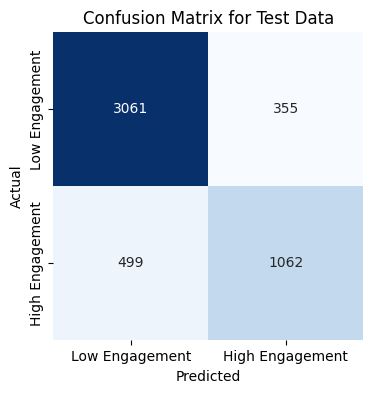
\includegraphics[width=\linewidth]{plots/binary_dt_confusion_matrix.png}
%         \captionsetup{justification=centering, width=0.9\linewidth}
%         \caption{Confusion matrix for binary classification}
%         \label{fig:conf_matr_binary_dt}
%     \end{minipage}
% \end{figure}

\subsection{Model Comparison - Binary Classification}
After having performed the task using the three algorithms, some interesting aspects emerged.
As expected, all the models, to a different extent, struggle to identify the minority class, \textit{High Engagement}, resuling in lower recall values
- 0.65 for K-NN, 0.70 for Naïve Bayes, and 0.68 for Decision Trees.
This is evident in the confusion matrices, where a significant number of \textit{High Engagement} records are misclassified as \textit{Low Engagement}.
In particular, K-NN handled the minority class the best in terms of precision and F1-score, achieving respectively 0.83 and 0.73.
However, the fact that Naïve Bayes performed better in terms of recall (0.70) makes it a more valid alternative
in scenarios where preventing high-engagement titles from being misclassified as low-engagement ones is a priority.
Decision Trees are located in the middle, showing similar performances to Naïve Bayes, but having a slightly lower recall.
In conclusion, considering all these aspects, K-NN is still considered the most efficient model for this task, as it also performs best globally. 
In the table~\ref{tab:best_model_binary_classification} its overall results are summarized.
\begin{table}[H]
    \centering
    \begin{tabular}{cccc}
        \toprule
        \bf{Accuracy} & \bf{Precision Macro Avg} & \bf{Recall Macro Avg} & \bf{F1-score Macro Avg} \\
        \midrule
         0.85 & 0.84 & 0.79 & 0.81 \\
        \bottomrule
    \end{tabular}
    \caption{Overall metrics - K-NN}
    \label{tab:best_model_binary_classification}
\end{table}





% \begin{table}[H]
%     \centering
%     \begin{tabular}{lcccccc}
%         \toprule
%         \bf{Model} & \bf{Precision} & \bf{Recall} & \bf{F1-score} & \bf{Accuracy} \\
%         \midrule
%         K-NN (Low Eng) & 0.83 & 0.65 & 0.72 & 0.85 \\
%         K-NN (High Eng) & 0.87 & 0.94 & 0.89 & 0.85 \\
%         \midrule
%         Naïve Bayes (Low Eng) & 0.74 & 0.70 & 0.72 & 0.83 \\
%         Naïve Bayes (High Eng) & 0.87 & 0.89 & 0.88 & 0.83 \\
%         \midrule    
%         Decision Tree (Low Eng) & 0.86 & 0.90 & 0.88 & 0.84 \\
%         Decision Tree (High Eng) & 0.75 & 0.68 & 0.72 & 0.84 \\
%         \bottomrule
%     \end{tabular}
%     \caption{Binary classification - performance comparison}
%     \label{tab:binary_classification_comparison}
% \end{table}





%%%%%%%%%%%%%%%%%%%%%%%%%%%%%%%%%%%%%%%%%%%%%%%%%%%%%%%%%%%%%%%%%%%%%%%%%%%%%%%%%%%%%%%%%%%%%%%%%%%%%%%%%%%%%5555
\section{Multiclass classification}\label{sec:multiclass_classification}
Among the multiclass features in the training set, \texttt{titleType} was selected as the target variable
for this task, due to its relevance within the dataset. Because of their strong correlation with
\texttt{titleType}, the feature \texttt{canHaveEpisodes} and the genre \textit{Short} were excluded from the
feature set. Furthermore, since the primary imputation method for missing values in \texttt{runtimeMinutes}
relied on information from the target variable, these values were re-imputed to avoid data leakage.
Specifically, missing entries were filled by sampling from the overall distribution of
\texttt{runtimeMinutes}, without referencing \texttt{titleType}.\\

One final point to note is the imbalance in the target feature (previously shown in
figure~\ref{fig:titleType_distrib}), which was explicitly taken into account
during the design of the models. As for the binary classification task, macro-averaged F1-score was
a key metric for model evaluation, as it provides a balance between each class's precision and recall.



% This feature was created to impute the missing values of the original \texttt{runtimeMinutes} variable,
% but without using the median value according to the titleType. Instead, the missing values were imputed using the help of two variables: \texttt{canHaveEpisodes} and \texttt{is\_Short}
% (as one of the resulting variables of the multi-label one-hot encoding process of the \texttt{genres} attribute).
% In particular, 
% \textbf{SCRIVERE COME E' STATA IMPUTATA NO\_TT - con canhaveepisodes e is\_short preso dai generi}.
% This approach prevents a significant error, as it would be methodologically incorrect to use \texttt{titleType}-based 
% imputation for an attribute when \texttt{titleType} itself is the target variable to predict.
\subsection{K-NN - Multiclass Classification}
For the multiclass classification task using the K-NN algorithm, the inclusion of a broad set of 
features is necessary and justified, as it was found to help the model to better distinguish between 
underrepresented classes - even if the results in their classification are not optimal. 
Even though this choice lowers the overall performance (accuracy) of the model, 
it is a trade-off in favor of larger coverage and sensitivity across all classes.\\
The hyperparameter tuning strategy that was employed is the same as in binary classification with K-NN. 
The configuration that achieved the best performances is: \texttt{{weights:'uniform', n\_neighbors:12, metric:'cityblock'}}.\\ 
As expected, the model shows mixed performances across the different classes. 
The overall test accuracy reaches 0.76, which is a respectable result for a multiclass problem. 
However, since accuracy is a global metric, more attention should be paied to the performances of the single classes. 
Classes with a larger support, like \textit{tvEpisode} (1596) and \textit{movie} (1848), are handled quite well: \textit{tvEpisode} reaches an F1-score of 0.83 and \textit{movie} 0.84, both supported by high recall values (respectively 0.93 and 0.87). 
\begin{figure}[H]
    \centering
    \begin{minipage}[t]{0.59\textwidth}
        \vspace{0pt}
        \small
        This is also clearly visible in the confusion matrix of Figure~\ref{fig:multiclass_knn_confusion_matrix}, where these classes dominate with a high count of correct predictions. 
        On the other hand, the model struggles with 3 classes in particular: \textit{tvMiniSeries} and \textit{tvSpecial}, i.e. the classes with the least support (respectively 68 and 42). 
        In particular, \textit{tvMiniSeries} shows a very low recall (0.03), meaning that it is rarely correctly identified. 
        Similarly, \textit{tvMovie} is mostly misclassified, showing a low F1-score of 0.29.\\
        
        An interesting trend to notice in the confusion matrix is how records belonging to class \textit{tvSeries} are frequently misclassified as \textit{tvEpisodes}. 
        This is likely due to the similar nature between the two, as both refer to television content and often share overlapping characteristics, considering also that a tv episode is basically part of a tv series. 
        A similar confusion occurs between \textit{tvMovie} and \textit{movie}.\\

        To summarize, since the model achieves a macro average F1-score of 0.50, this reflects clearly this imbalance in performance: while the model performs well on the majority classes, it fails to generalize well especially the minority ones.
    \end{minipage}
    \hfill
    \begin{minipage}[t]{0.40\textwidth}
        \vspace{0pt}
        \centering
        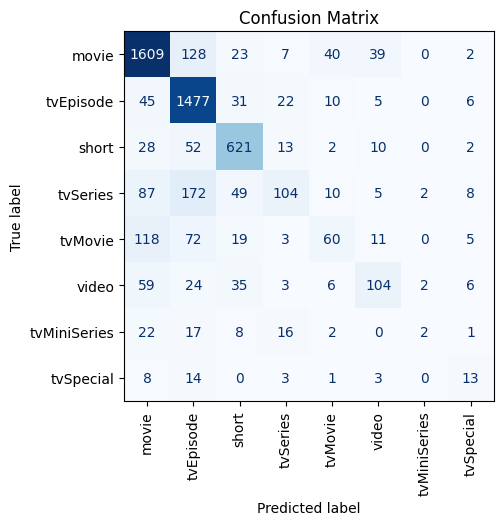
\includegraphics[width=\linewidth]{plots/knn_multiclass_confmatrix.png}
        \captionsetup{justification=centering, width=0.65\linewidth}
        \caption{K-NN multiclass classification}
        \label{fig:multiclass_knn_confusion_matrix}
    \end{minipage}
\end{figure}
\vspace{-0.8em}

% This is also clearly visible in the confusion matrix of Figure~\ref{fig:multiclass_knn_confusion_matrix}, where these classes dominate with a high count of correct predictions.
% On the other hand, the model struggles with 3 classes in particular: \textit{tvMiniSeries} and \textit{tvSpecial} , i.e. the classes with the least support (respectively 68 and 42). 
% In particular, \textit{tvMiniSeries} shows a very low recall (0.03), meaning that it is rarely correctly identified. Similarly, \textit{tvMovie} is mostly misclassified, showing a low F1-score of 0.29.\\
% \begin{figure}[H]
%     \centering
%     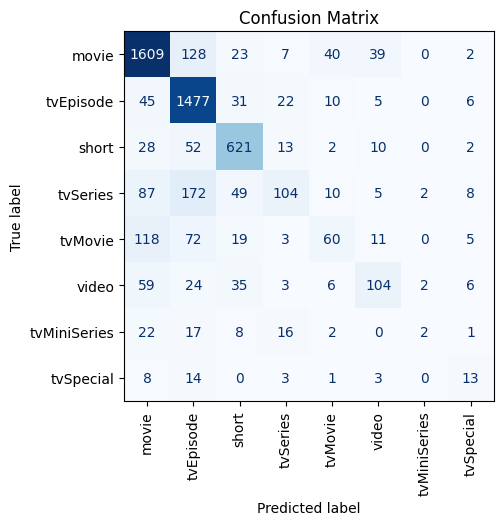
\includegraphics[width=0.45\linewidth]{plots/knn_multiclass_confmatrix.png}
%     \captionsetup{justification=centering, width=0.9\linewidth}
%     \caption{Confusion matrix - K-NN muticlass classification}
%     \label{fig:multiclass_knn_confusion_matrix}
% \end{figure} 
% An interesting trend to notice in the confusion matrix is how records belonging to class \textit{tvSeries} are frequently misclassified as \textit{tvEpisodes}. 
% This is likely due to the similar nature between the two, as both refer to television content and often share overlapping characteristics, considering also that a tv episode is being basically part of a tv series. 
% A similar confusion occurs between \textit{tvMovie} and \textit{movie}.\\



\subsection{Naïve Bayes - Multiclass Classification}    
Also for the Multiclass Classification task the features has been preprocessed as explained in paragraph X, 
in order to use Categorical NB. For this task it has been interesting to note that the inclusion of genre features enhanced classification performance 
for all classes but especially for the ones with limited support: tvMiniSeries (68 objects) was not classified at all and tvMovie (288) and tvSpecial (42) 
were poorly classified. This confirmed the choice of CategoricalNB over GaussianNB; being the first the most indicated to handle categorical features.\\
The model achieves an overall accuracy of 0.73, acceptable for a multiclass task but indicative of difficulties in handling all categories equally well. 
High F1-scores for the most represented classes—movie (0.83), tvEpisode (0.79), and short (0.81)—suggest effective recognition, likely due to their frequency in the dataset and the presence of more easily distinctive traits. The movie class also shows strong precision (0.82) and recall (0.84), 
confirming the model's reliability on this category.\\
As expected, performances drop significantly for underrepresented classes. tvMiniSeries (0.02), tvSpecial (0.21), and tvMovie (0.17) exhibit low F1-scores, indicating that the model has significant difficulties distinguishing correctly these examples. 
Other than their low support, this is probably linked to the presence of common features with more dominant classes, such as Movie or tvEpisode. This is supported by the confusion matrix, which shows, for example, tha 140 tvMovie instances are  misclassified as movie, highlighting a strong confusion between these two categories.\\
The tvSeries class also presents issues, with moderate precision (0.52) but a rather low recall (0.40): indicating many missed instances
To conclude, the very low F1 macro average score, actually reflects the inability of the model to perform in a balanced way on all the classes. 
On the other hand, the F1 weighted average results of 0.71, suggesting that the majority classes have a greater influence on overall performance than the minorities.
\begin{figure}[H]
    \centering
    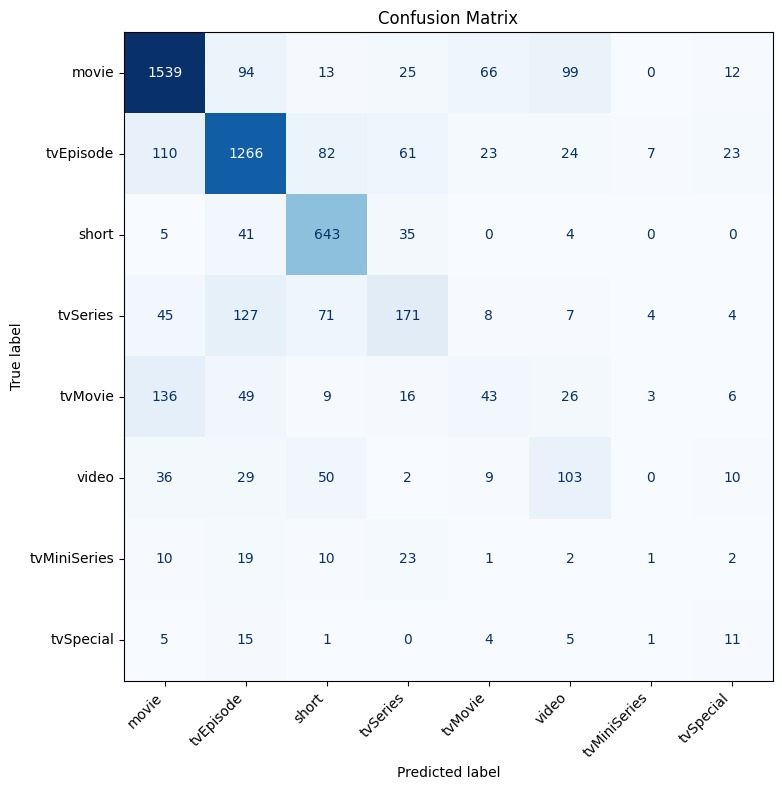
\includegraphics[width=0.30\linewidth]{plots/nb_multiclass_confmatrix.jpg}
    \captionsetup{justification=centering, width=0.9\linewidth}
    \caption{Naïve Bayes multiclass classification}
    \label{fig:nb_multiclass}
\end{figure}



\subsection{Decision Trees - Multiclass Classification}
Like for the binary classification task, the Decision Tree model was trained without normalizing or
transforming the features, making the model more interpretable. Feature selection was performed by studying
feature importance, while hyperparameters were optimized with a Randomized Search,
which used Repeated Stratified 5-Fold Cross-Validation with 5 repeats on the training set, optimized for
the macro-averaged F1-score.
The best configuration found used Entropy as splitting criterion, had a max depth of 14, a minimum of
5 samples per leaf, and a minimum of 8 samples in order to split an internal node.
\begin{figure}[H]
    \centering
    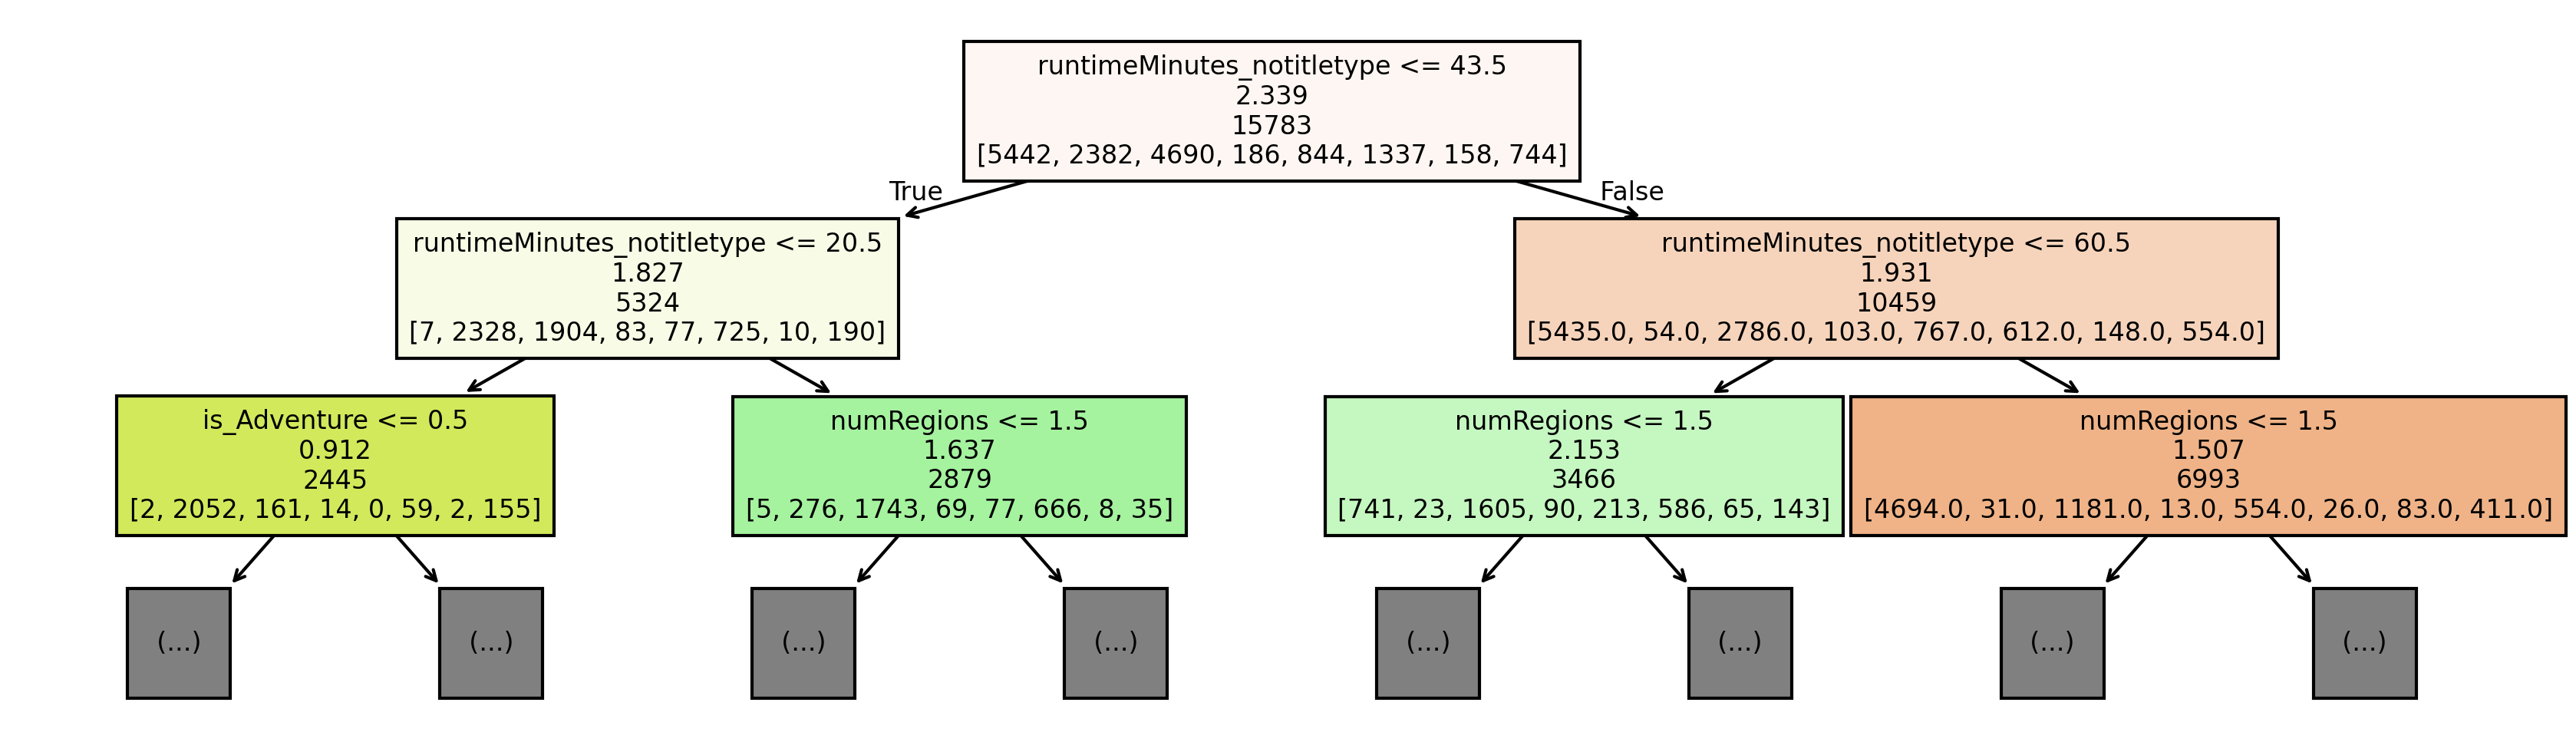
\includegraphics[width=0.88\linewidth]{plots/multiclass_tree.png}
    \captionsetup{justification=centering, width=0.9\linewidth}
    \caption{Decision Tree for multiclass classification}
    \label{fig:multiclass_dt}
\end{figure}

\begin{wrapfigure}{r}{0.4\textwidth}
    \centering
    \captionsetup{justification=raggedleft, width=1\linewidth}
    \caption{Confusion matrix for the model}
    \label{fig:multiclass_dt_conf_matrix}
    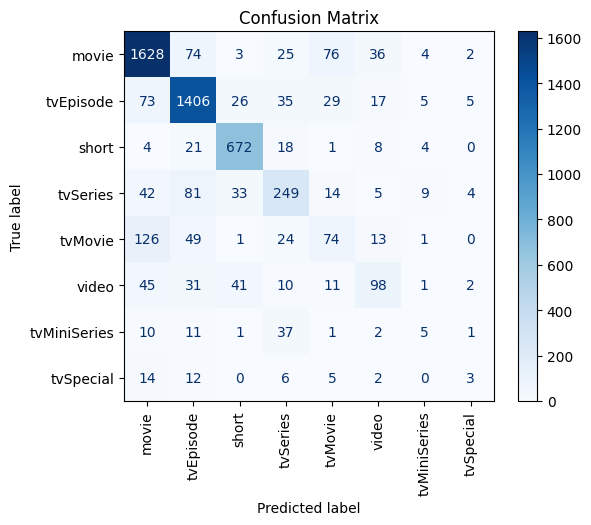
\includegraphics[width=0.9\linewidth]{plots/multiclass_dt_conf_matrix.png}
\end{wrapfigure}
Figure~\ref{fig:multiclass_dt} shows the Decision Tree obtained for the multiclass classification task.
The most important feature for the model was\texttt{runtimeMinutes}, on which the first two levels
of the tree are based, with a feature importance of 0.45.
Three out of the four splits in the following level are based on \texttt{numRegions} being smaller than
2, giving the feature an importance of 0.13; the fourth is based on the \textit{Adventure} genre,
which has an importance of 0.01.\\
The model showed a general tendency towards overfitting, and many configurations were tested to prevent
this.
The overall accuracy shows a significant drop (from 0.86 on the train set, to 0.75 on the test set),
as well the macro-averaged F1-score, going from 0.65 to 0.52.
This was given from the \textit{tvMiniSeries} and \textit{tvSpecial} classes: these had f1-scores of
0.35, 0.22 respectively on the train set, and both had 0.10 on the test set. Since they were by far
the least represented classes, they required a trade-off between low-represented classes classification
and generalization. This can be seen in figure~\ref{fig:multiclass_dt_conf_matrix}, which shows the fact
that most predictions for these classes were misclassified.\\
In order to mitigate overfitting, post-pruning was tested, but did not give particular benefits.
Higher values for the parameter $\alpha$ had minor positive effects on the generalization
capabilities of the models, at the cost of losing predictions on the less represented classes.
Another aspect highlighted by the confusion matrix is the fact that \textit{tvMovie} was often
classified as \textit{movie}, leading to a Recall value of 0.26 on the test set.
This is likely due to the fact that the two classes are overlapping, since they are semantically related,
and is further supported by the fact that the most common misclassification for \textit{movie} was
\textit{tvMovie}, albeit with a low number of occurrences, likely due to it being the biggest class.
A similar case can be made for \textit{tvSeries} and \textit{tvMiniSeries}, with 37 out of the total 68
of the \textit{tvMiniSeries} records being misclassified as \textit{tvSeries}.



\subsection{Model Comparison - Multiclass Classification}
Because of class imbalance, for evaluation purposes,
macro-averaged F1-score was heavily considered.